\chapter{Simulation}
\label{simulation}
\epigraph{A model is a physical, mathematical, or logical representation of a system entity, phenomenon, or process. 
A simulation is the implementation of a model over time. 
A simulation brings a model to life and shows how a particular object or phenomenon will behave.}
{\textit{Systems Engineering Fundamentals. Defense Acquisition University Press, 2001}}

In the previous chapters \modelname has been used to represent CSE.
A \modelname instance can represent any evolution of a component system.
However, as a goal of this research is to simulate CSE, realistic component evolutions are necessary.
This chapter presents a conceptual model that can be used to generate realistic component system evolutions.

This chapter first describes the reason that a simulation has been chosen as the method to study CSE.
Simulation is compared to other types of possible avenues of study, looking at real systems and users or using a controlled environment.
Then the methodology outlined by \cite{Law2005} is described, 
and its core artifact, the ``conceptual model'', is discussed.

A user survey is then presented.
This survey was used to construct the conceptual model, by studying how a user evolves their componetn systems.
This survey focused on users of package managers, to evolve GNU/Linux operating systems.

Finally, this chapter describes the conceptual model, and how this model can be used to create CUDF* documents that describe realistic component system evolutions. 
Such a CUDF* document can then be resolved by GJSolver, and the resulting systems studied.
These relationships are described in figure \ref{sim.modeldiagram}.

\begin{figure}[htp]
\begin{center}
\digraph[scale=.5]{simmodeldiagram}{
rankdir=BT;
CMS[label=<<TABLE BORDER="0" CELLBORDER="1" CELLSPACING="5"><TR><TD WIDTH="150">CUDF*</TD></TR></TABLE>> shape=none];
subgraph {
	rank=same;
	CMI[label=<<TABLE BORDER="0" CELLBORDER="1" CELLSPACING="5"><TR><TD WIDTH="150">:CUDF*</TD></TR></TABLE>> shape=none];
	ConMI[label=<<TABLE BORDER="0" CELLBORDER="1" CELLSPACING="5"><TR><TD WIDTH="150">:Conceptual Model</TD></TR></TABLE>> shape=none];
}
ConM[label=<<TABLE BORDER="0" CELLBORDER="1" CELLSPACING="5"><TR><TD WIDTH="150">Conceptual Model</TD></TR></TABLE>> shape=none];
CMI -> CMS [ label="instantiates"];
ConMI -> ConM [ label="instantiates"];
ConMI -> CMI [ label="creates"];
}
  \caption[labelInTOC]{figureCaption}
  \label{sim.modeldiagram}
\end{center}
\end{figure}


\section{The Study of Component System Evolution}
To study the CSE process, many component systems change in response to requests must be studied.
These evolutions consist of a series of component systems that are snapshots before and after a requested change.
To obtain this information three methods could be used:
\begin{enumerate}
  \item field data could be collected from real systems evolving ``in the wild''.
  \item a controlled environment could be created, in which systems are monitored as users are asked to request changes.
  \item a simulation of a systems evolution could be run, where variables of the simulation are altered to represent different environments and situations.
\end{enumerate} 

In this section the positive and negative aspects of each of these approaches are discussed,
and the reasons for the selection of the simulation method for this research are presented.

\subsection{Using Real Users and Systems}
Studying real systems that are evolved by real users is one method of studying CSE.
Users could participate by installing monitoring software in their component systems that collects data.
This data could then be used to study the process by which their systems evolve.

This approach  has significant drawbacks:
\begin{itemize}
  \item it will take long periods of time to find meaningful results.
  \item the monitoring of user's actions is an invasion of their privacy, which may limit the pool of willing participants.
  \item finding and convincing enough users to participate to generate useful results will require significant effort.
\end{itemize}

\subsection{Users in a Controlled Environment}
To increase the efficiency of collecting results and to eliminate privacy issues of users, a controlled environment may be created.
Such an environment could be created in a laboratory setting, and consist of a component system and a participant.
This participant would then be asked to evolve the system to approximate their real actions, where the resulting systems could then be studied.

Such a controlled environment could very quickly simulate  many interactions that would of occurred over a long period.  
It also removes the necessity user trust as the user is altering a system that is not theirs.
However, it will also produce less valid results, as it is still an approximation of a real system, and the users know this.
Any controlled environment would alter how the user interacts with their controlled system, making the results less reliable.

However, the largest problem with this method is the effort required to conduct the experiment on enough users to find significant results.
The core difficulty with this method is finding and convincing enough users to participate, and then monitoring and supporting them while they are in the controlled environment.

\subsection{Simulating the Problem}
CSE can be studied by simulating the users actions and the component system using reasonable approximations.
A simulation is a surrogate of the real system, 
such that it represents the core aspects of the reality while simplifying and abstracting away unnecessary detail.
The goal of a simulation is not to represent every aspect of the real world, 
but to make a ``close enough'' approximation so that the conclusions drawn from it are valid while minimising complexity.

When analysing the results and forming conclusions from a simulation, 
the assumptions and abstractions made, must be taken into account.
Therefore, the majority of the effort of creating a simulation is making sure the results from the simulation are valid.

\subsection{Why Simulate?}
The advantages of simulating are the speed at which ideas can be tested and evaluated;
the cost to test and get results; and the control over variables and configuration of the environment.

The core steps to generate new knowledge is the iterative process of creating a hypothesis, then testing its accuracy.
As the speed of this process increases, the greater amount of knowledge and meaningful information that can be generated. 
Using real users, or real systems, requires long periods of waiting and preparation where little or no progress is made.
However, if the actions and environment can be modeled and executed computationally, these times of no progress are eliminated.

%%%Cost
The cost of testing a hypothesis can be measured in the amount of time it takes to define an experiment and to collect the results.
Using real users requires significant amount of time to collect and convince users to participate.
However, with a simulation the main effort is ensuring that the returned results are valid.
Once the simulations validity is established, it takes very little time to test a hypothesis.

%%%Control
The control over the variables in a simulation allows for testing extreme and normal situations.
It also allows for the sensitivity analysis of different variables, finding how important they are to the simulated system.

%%%Final words on why we simulate
A simulation of CSE is selected in this research as it has a cost/benefit ratio that is desirable,
and provides an acceptable level of accuracy to draw meaningful conclusions.

\section{Methodology}
%%%We use the methodology from `` Build a Valid and Credible Simulation''
The core hurdle in creating a simulation is validating the returned results are similar to reality.
To create a valid and credible simulation the methodology that \citep{Law2005} outlines is followed.
This methodology is a guideline for defining the study, collecting information, creating and validating models, and running the simulation.
In this section the methodology is described and aligned to this research's objectives. 

\subsection{Validation and Credibility}
%%%Why do we use this methodology and how is it relevant?
This methodology was created after the observation that validation was often ``attempted after the simulation models had already been developed'' \citep{Law2005}.
That is even if validation was attempted, it may only occurred if there was money and time left at the end of the project.
However, such simulations, that are not validated, can produce erroneous information that leads to bad, possibly costly decisions being made.
This reduces the credibility of the simulation to be used in future as a tool.

A simulation is an abstraction and simplification of reality, often created as using an actual system can be disruptive, not cost-effective, or simply impossible.
In this context,

\begin{quotation}
``\textit{Validation} is the process of determining whether a simulation is an accurate representation of the system, for the particular object of the study.'' \citep{Law2005}
\end{quotation}

The latter part is an important aspect of validation, as the accuracy of the simulation is directly dependent on the problem and questions the study addresses.
Therefore, the definition of the problem will directly lead to the modelling and scope of the simulation.

%%%What is credible
A simulation, and by extension its results, have \textit{credibility} if key stakeholders accept them as ``correct''.
A credible model is not necessarily valid, and vice-versa, as it involves the input of a person who decides if the goals of the simulation have been obtained.
Credibility of a simulation is then only attainable if the key personale from the project understand and are involved directly with the project.

The simulation produced by this study to identify the effect of different strategies on the evolution of component systems must be validated to produce meaningful results,
and must be credible for these results to be trusted.

\subsection{Seven Step Method}
The methodology presented in \citep{Law2005} has a seven step approach to creating a valid and credible simulation.
These steps are; formulating the problem; collecting information and data to construct a conceptual model; validating the conceptual model;
implementing (programming) the model; validating the programmed model; designing, conducting and analysing experiments; and documenting and presenting the simulation results.

\subsubsection{Step 1: Formulate the problem}
The first step is to formulate the problem as clearly as possible, this is usually done with core stakeholders in a ``kick-off meeting''.
The core artifacts from this step are the overall objectives of the study, specific questions wanting to be answered, scope of the study,
 and different configurations of the simulation with the measures used to evaluate their performance. 

\subsubsection{Step 2: Collect information and data to construct conceptual model}
The conceptual model is a description of how the simulation and system work relative to the problems earlier defined.
It is the most important artifact of the simulation.
It should be high level enough to be understood by the core stakeholders but detailed enough to be reused in future simulations.
It is created through interviews with subject matter experts and collecting relevant data like results from similar exiting systems.
Problems like the data not being representative of the model, not being in the appropriate format or type, and containing errors must be handled before use.

The conceptual model also contains all of the variables that can be configured including their documented assumptions. 
It is defined to the level of detail with respect to project objectives, performance measures, data availability, computer constraints, and resource constraints.

\subsubsection{Step 3: Conceptual model validation}
The conceptual model is the most important aspect of the simulation, thus its validation must be thorough.
The core method used to validate this model, is to discuss it with core-stakeholders and subject matter experts.
This provides feedback as to the direction of the conceptual model, ensuring that it will answer the questions posed in the study.

\subsubsection{Step 4: Implement the conceptual model}
The implementation of the conceptual model must also be executed and documented in a way that allows others to replicate and repeat the process.
The artifacts created during this process must be verified to work correctly, this can be accomplished through test-cases and debugging \citep{Pressman1992}.

\subsubsection{Step 5: Validate implementation}
There is no completely definitive approach to validating the simulation,
however, the most definitive test of a simulations validity is established by closely looking at the outputted results compared to that from an actual system \citep{Law2005}.

This is done through:
\begin{itemize}
  \item \textbf{Results validation: } a comparable system is used to create results and compared with the results from the simulation for validation.
  \item \textbf{Face Validation: } experts are given output of the simulation model and checked to see if it is consistent with how they perceive the system should operate.
\end{itemize}

Further validation of the implementation can be accomplished with sensitivity analysis,
which is performed on the simulation to find the factors with the greatest impact on the performance and results.

\subsubsection{Step 6: Design, conduct and analyse experiments}
For each of the experiments that are run, the time and number of independent runs must be defined.
If the results are inconclusive, or other aspects of interest have arisen, it may be necessary to run additional experiments.

\subsubsection{Step 7: Document and present results}
This step involves the presentation of the conceptual model, simulation, and results to the core-stakeholders.
This presentation is critical for the future re-use of the model, as it should promote credibility through describing the validation process.

\subsection{Differences in methodology}
A core goal of creating this simulation study is to produce valid and credible results.
However, this specific methodology has been created for large scale industrial projects with substantial resources.
As this study is smaller in scale and resources some of the procedures recommended in this methodology have been restricted and some removed.

The most significant difference between this study and the described methodology is the clear definition between decision-maker and simulation designer.
In larger projects a simulation designer is contracted by a decision-maker who has a problem to solve or question to answer.
In this project both these people are the same person, therefore meetings between them are not required.

Other people in the project including subject-matter experts, core-stakeholders, simulation analysts consist of survey participants and project supervisors.
This is because the limits of the projects resources excludes the employment of experts for validation.
This may reduce the validity of the end model, but these restrictions have been made only when necessary,
and done so in a manner that attempts to minimise negative effects.


\section{User Survey}
\label{strat.usersurvey}
To explore the users role in CSE and to construct a conceptual model, a survey was given to users.
The previous chapters have left the role a user plays in the evolution of their component system unexplored.
This section describes the motivations and strategies for users to evolve their component systems.

A strategy is the plan or pattern employed by a user to evolve a system.
A fundamental influence on the user's strategy is their perception of risk.
Each change to the system the user requests, and the criteria used to accomplish this change is effected by the risk of that change.
For example, upgrading a system may introduce new bugs and problems, yet not upgrading may let old vulnerabilities compromise the system.

%%%The survey used to validate and refine the model
This survey targeted users of GNU/Linux distributions (specifically Ubuntu), and server administrators through the online forum reddit\footnote{http://reddit.com accessed 6/3/2012}.
In this context the way in which component systems are evolved is through package managers, as described in chapter \ref{background}.
It was completed by 59 users, who answered questions about themselves, the system they are evolving, and the way in which they evolve it.
It also optionally involved the submission of package manager log files, which through analysis can provide greater detail of user behaviours.
These logs are not analysed here, but are used further discussed in chapter \ref{ubunutsimulation}.

In this section a brief description of the survey and an analysis of responses is given.
The full set of questions in the survey is presented in section \ref{apx.survey}. 

\subsection{Questions}
%%%The goals of the survey:
There are two types of questions in the survey; a set to identify the type of user, and a set to describe their interactions with package managers.

A set of questions used to identify the user are:
\begin{itemize}
  \item How experienced with package managers are you? 
  \item What system are you using?
  \item What package manager are you using?
\end{itemize}
These can be used to categorise the type of user and put into context the answers that they give.
They can also be used to weigh their answers for credibility and potentially exclude results from novice or inexperienced users. 

A set of questions asked about their use of package mangers are:
\begin{itemize}
  \item Describe your initial interaction with the package manager.
  \item Describe your day to day interactions with the package manager.
  \item What usage life cycle do you have with the package manager?
  \item Describe an unusual scenario in which the package manager was used.
\end{itemize}
The main focus of these questions is to identify the life-cycle of interactions that the user has when evolving a system.
The responses will provide reasons for these actions to occur, and illuminates the users objectives and strategies.

The survey finished with the question:
\begin{itemize}
  \item What other questions should I have asked?
\end{itemize}
This question tried to illicit comments and possible information that could of been gathered.
It also provided a minor verification of the survey, as to see if anything was missing that should of been asked.

\subsection{Results}
%%%The results are summarised as:
The type of user that submitted the survey is important to be able to put in context their replies.
Most users (29/59) used the dpkg component model, either in Debian or Ubuntu systems.
The majority of these users used apt-get as their package manager.
The next largest component model used was ArchLinux\footnote{http://www.archlinux.org/ accessed 6/3/2012} (13/59),
all using the package manager pacman\footnote{http://www.archlinux.org/pacman/ accessed 6/3/2012}.
Other represented component models and package mangers include, Fedora with the rpm component model and the yum package manger,
Slackware with pkgtools, and Gentoo with portage.

The users mean experience was recorded as 3.9/5.
This is a subjective measure, but it describes the confidence in which the participants answered the questions. 

The life cycle questions have been summarised into the frequency of each action in table \ref{strat.tblaction}.

\begin{table}[htp]
\begin{tabular}{l | c | c | c | c |}
Request & Init. & Daily & Weekly & Monthly \\
Upgrade  & 45 & 27 & 16 & 0 \\
Install & 49 & 6 & 17 & 3 \\
Remove & 6 & 4 & 1 & 0\\
\end{tabular}
\caption{Summary of the frequency of user actions with package managers}
\label{strat.tblaction}
\end{table}

This table shows the amount of users from the survey who perform the actions of upgrading their system, installing or removing a package 
initially (when the system is first created), daily, weekly or monthly.
It shows that the vast majority of users when they create a system upgrade the system and install required packages.
This also shows that most users upgrade their system daily, and if they will likely install a package weekly.

The unusual scenarios which the user described using the package manager included 
11 of the 59 users stating that they had installed a set of packages to fulfil a specific task only to remove them almost immediately.
This is described by the users response 
\begin{quote}
``I sometimes install lots of packages very quickly as I need to accomplish a task, then remove them once that task has finished.''
\end{quote}

Also, 3 of the users stated that the package manager broke their system at some point, which then required to be fixed through the package manager.

In the final question asked if there is any more questions the general themes of responses include:
\begin{itemize}
  \item the mitigation of failed actions
  \item installing multiple versions of packages
  \item using a graphical user interface v.s. console based package manager
\end{itemize} 
The majority (37/59) users did not fill out this option in the survey, a potential indicator that the survey was complete.
One user even remarked to this question:
\begin{quote}
``Quite an all encompassing survey!''
\end{quote}

\subsection{Progressive vs. Conservative Users}
The main outcome of this survey was the identification of different user strategies towards evolving a component system.
These strategies have been used to defined into two user stereotypes, \textbf{conservative} and \textbf{progressive}.
These terms come from the domain of politics where conservatism is the philosophy that emphasises minimal and gradual change in society,
where progressivism promotes change and reform.
These strategies can be caused because of a conflicting perception of risk; the risk of change introducing new problems, and the risk of not changing having old problems persist.

Most users in the survey are between these two strategies. 
For example, a users response that express a slight conservative attitude:
\begin{quotation}
In production I rarely remove packages (easier to leave software as-is than risk breaking stuff).
\end{quotation}
That is they are more likely not to change the system, even though it may be beneficial as it may lead to a fault. 

Another example of a users response expressing a slight progressive attitude:
\begin{quotation}
I update my packages whenever I log in each day
\end{quotation}
Upgrading the system each day will ensure that no packages with fixed bugs will be installed, though may require significant change.

Both of these strategies have extremes though, where users who try to eliminate all of a risk.

For example, a user's response in the survey with an extreme progressive attitude:
\begin{quotation}
I do run an unstable system all the time, I help mitigate this with some redundancy in my most frequently used components, 
using packages which perform the same function, but have different dependencies, since it's less likely to have multiple packages break at the same time. 
If something is rather buggy for me, I tend to update on a more frequent basis to check for the next stable point to jump into.
\end{quotation}
This user has components in their system that are so new as to not be fully tested, which are described as unstable packages.
To lower the risk that such packages have on the function of the system, this user has redundant functionality installed in their system to ensure that it can be used.
This users system will almost certainly be completely up to date, as any new component versions will be immediately integrated into their system.

An example of an extremely conservative user's response when asked about the frequency with which they interact with the package manager:
\begin{quotation}
As little as possible. I like build my box into whatever I'll need in the first couple of weeks after an install. 
Following the configuration and construction, only the occasional upgrade is necessary. 
Unless, of course, I receive a security notice about something.
\end{quotation}
So after the setting up of a system, this user will not evolve the system unless there is a direct security risk.
This lack of change will result in the system quickly becoming out of date.

%%%The reasons for keeping a system up-to-date; the fixing of bugs security, the adding of functionality, 
The reasons for these progressive attitudes of users is that maintaining an up-to-date system will eliminate known security exploits against the system,
and also introduce more efficient or new functionality into the system.
%%%The reasons for minimal change; through change unknown bugs could be introduced, the act of changing can create bugs, the effort of changing can consume resources  (e.g. network traffic).
Where the conservative attitudes come from the wither the perceived risk that unknown bugs could be introduced into the system, the act of changing a system can cause faults,
or the consumed resources (e.g. time, network traffic) are to expensive compared to the benefits.

Both concerns are valid assessments of the risk of component system evolution, the user must decide with respect to their system, what strategy to employ. 
For example, a server administrator that is running a mission critical system will likely change the system begrudgingly as any fault could cause massive damage.
However, a user running a desktop personal computer system may be more interested in new functionality, so would change more readily.

\section{Conceptual Model}
In this section the ``conceptual model'' of the component system evolution process is presented.
The conceptual model is defined to represent \textbf{realistic} component system evolutions.

This relation to reality is the core difference between the conceptual model and the \modelname model.
For example, \modelname could describe a situation where a user may requests to upgrade their system every minute for a year.
This situation is clearly unrealistic, and not able to be represented by the conceptual model.

In this section, the conceptual models of the user and components are described.
How an instance of the conceptual model can be used to create a realistic component system evolution, represented by a CUDF* document, is also described.

\subsection{Conceptual User}
The core aspect modeled by the conceptual user is what and when requests will made to change the system. 

In CUDF* three different actions are defined that a user can request to alter their system; installing, removing or upgrading a component.
However, as shown in the user survey presented in chapter \ref{strategies} the two main actions of users are the installation of a component, and the upgrading of the entire system.
The daily level has been selected as the frequency of these actions, as this is a reasonable time period expressed often in the user survey. 

%%%We have limited it to two actions, install and update, as they are the core actions a user executes
The variables that make up the conceptual user are: 
\begin{itemize}
  \item $u$ is the probability a user requests to update the system per day.
  \item $i$ is the probability a user requests to install per day.
  \item $\mathbb{N}_p$ is a set of component names where for each name $n$, $n_p$ is the probability that a component with name $n$ will be requested to be installed.
  The sum of all probabilities equals 1.
  \item $U$ is the MOF criteria used to select an optimal system for an update request.
  \item $I$ is the MOF criteria used to select an optimal system for an install request.
  \item $d$ is the number of days requests are made.
\end{itemize}

To illustrate the use of this model, consider the example where:
\begin{itemize}
  \item $u =.2$
  \item $i =.2$
  \item $\mathbb{N}_p = \{n,m\}$ and  $n_p = .25$ and $m_p = .75$
  \item $U = $ \texttt{-removed,-new,-uptodatedistance}
  \item $I = $ \texttt{-removed,-changed,-uptodatedistance}
  \item $d = 20$
\end{itemize}
The variables $u$ and $i$ equal $.2$, this means that on any day the user has a 20\% probability of requesting to upgrade and/or install a component.
If a user requests to install a component, the component name $n$ has a 25\% probability of being selected, and the component name $m$ is 75\% likely. 
When the system is selected to be upgraded, the most criteria used is $U$, whose most important criterion is to minimise the amount of removed components.
The install criteria $I$ is similar to the update criteria, except that is minimises all change to the system.
Finally $d$ describes how many days this user will potentially request for, which is $20$.

Using this model it can be expected that there will be $4$ requests to upgrade the system and $4$ requests to install a component.
Component names  are selected to be installed without replacement, i.e. the same component name cannot be selected twice to be installed.
Therefore, only $2$ requests to install can be made, and it is expected that name $m$ will be selected first.


\subsubsection{Discussion of Conceptual User}
This section presents a brief discussion about the conceptual user compared to the users from the survey.

The conceptual user does not model the initial requests made when the system is new, 
or the discussed pattern of installing then removing packages.
The reason for not including these elements in the model is to maintain the simplicity of this model.
Including these actions into the user model would dramatically increase the complexity of the model, 
which might overshadow the core element being modeled. 

One request made by the user in reality may impact the occurrence of another action, so that they are correlated to happen together.
For example, a user may select to always update before they install, or to select a component to be installed because of another installed component.
The complexity that can be introduced by these correlations could make this simulation impractical.
For the practicality of the simulation, and the simplicity of the presented models, the corrolation between requests is ignored.

\subsection{Conceptual Components Model}
The only item that is necessary in the conceptual component model is 
a partial CUDF* document that includes the preamble, and package stanzas that can be parsed to create the time $t_0$, the initial system $\alpha_{t_0}$ and the set of components $C_{t_0},\ldots,C_{t_n}$.
This document is complete with the exception of the user requests that will be generated using the conceptual user model.


\subsection{CUDF* Document Creation}
The main goal of the conceptual model is to create realistic component system evolutions represented by CUDF* document.
This section presents the process to generate a CUDF* document from an instance of the conceptual model. 
A CUDF* document generated by this process can then be used to 


\section{Simulation Validation}
%%%Validation of this simulation, what needs to be validated/why it should be validated
The conceptual model presented is a simplified abstraction of the reality in which users evolve component systems.
It describes the variables that effect component system evolution as a configuration,
and the processors used to execute the simulation given a configuration.

%%%What if it is wrong
If some significant aspect of the system was missed, or if some aspect was incorrectly defined, the simulation may produce results that are incomprehensible,
or worse, misunderstood.
Therefore, the validation of these artifacts is essential to move forward. 
This validation was accomplished though regular stakeholder meetings, and an online survey with subject matter experts (as described in chapter \ref{strategies}).

\subsection{Stakeholder Meetings}
%%%Weekly meetings with stakeholders (i.e. supervisors)
As described in the methodology; one effort to validate these artifacts is done through meetings and a structured walk-through with the core stakeholders.
In this simulation the core stakeholders are the project researcher and supervisors.
These are the people who are asking the questions and are also impacted by the outcome, therefore they are directly effected by the validity of the results.
Meetings where held at regular intervals to ensure the projects progress and direction where correct.

\subsection{Subject Matter Expert Survey}
%%%Results from what else should be asked, install stuff not from repository, installs break
The survey described in chapter \ref{strategies}, 
was conducted at a point in the project when the conceptual model was just being developed, so had considerable impact on these artifacts.
The questions asked in this survey helped gauge the necessity and frequency of user actions,
so that only the most important aspects of the problem can be selected to be simulated.
It also filled in gaps of what was missing from the survey and model, giving direction for exploration.

\subsubsection{Frequency of User Actions}
%%%How often do users do these actions
The more frequently a user selects an action to evolve their system, the more important it is to the evolution of their system.
The information gained from the survey provides confidence that not including the action to remove a component and abstract the requirement multiple repositories, 
would not damage the validity of the results.
It also helped us define and represent the update and install actions in the configuration.

The remove action can be ignored as it seemed many of the users do not use this frequently.
When they do select to remove a component it is usually directly after installing it, if the selection to install a component was seen as a mistake.
Although it is clearly an important function to be included when evolving a system, the assumption is made that it is unnecessary for this simulation.

This survey also clearly shows that the main actions of a user is to update their system,
with the installation of a component the second most used action.
This survey also showed that the update occurs at more regular intervals than the install components.
Therefore, only the update and install user actions were included in this simulation and it also defined their representation. 

\subsubsection{Component Fault Exploration}
Another aspect of this problem that was mentioned by the subject matter experts through the survey was that a system may break during a change.
This typically then requires a reversion of the system components to a previously stable state.
Simulating this effect was ultimately deemed outside the scope of the project as it is seen as a rare occurrence with modern systems.
However, before it was eliminated, it was explored for possible inclusion.

The core problem with including simulated faults in a component systems evolution, is that each component has a different likelihood of causing a fault.
Different properties of a component like development process or complexity can impact this value.
Therefore, the function to calculate the likelihood of a component failing could rely on many different properties.

Instead of creating a function that tried to calculate the probability of failure per component,
an effort to measure it was attempted through a small study of component bug reports was attempted.

The feedback generated when a component causes a fault should ideally be a bug report, for the Ubuntu distribution these are filed on the project hosting server LaunchPad.
By using the Launchpad API to extract bug information, the amount of bugs per component in the system was able to be measured.
It was initially assumed that the number of systems that a component was installed on would increase the number of bug reports generated,
as more users means more eyes and systems to find bugs.
The Ubuntu Debian popularity contest was used then to see if this relationship existed the graph in figure \ref{bugsvspop} was created.

\begin{figure}[htp]
\begin{center}
  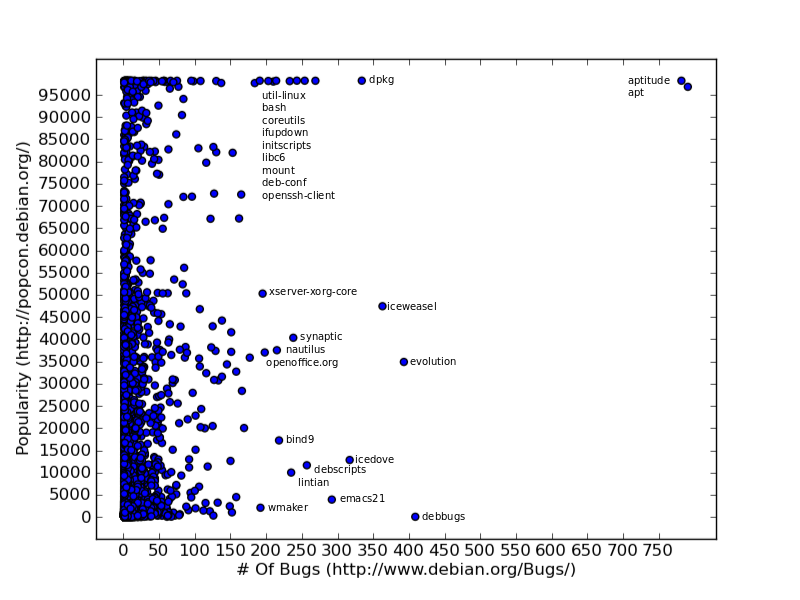
\includegraphics[width=\textwidth]{simulationpics/bugsvspopularity}
  \caption[Bugs v.s. Popularity]{A plot of the bugs a package has compared to its popularity, with notable outliers labeled}
  \label{bugsvspop}
\end{center}
\end{figure}

The first thing to note is that there seems to be very little relationship between the two variables, other than the package with the most bug reports is also one of the most used components.
The second thing to note is that the packages with the largest amount of bugs are ``apt'' and ``aptitude'' the two most popular package managers.
This could be because those packages are very buggy, or it could be because problems caused by apt, e.g. trying and failing to install a faulty package, may be reported as a problem with apt.

The last thing to notice is that there are many less popular components that have many bug reports.
When identifying the purposes of these packages many are used by developers, e.g. emacs21 is a popular text editor to program in.
The reason for their increased amount of bug reports may be that the users have prior experience and appreciation for the bug reports and the maintenance process, so file more bugs.

Measuring a components likely hood of failure using bug reports is then hypothesised to be impractical if not impossible,
as a component purpose and a components users may affect the results of the best measurement method available.
Other methods of finding a components likelihood of failure have not been further explored since this variable was eliminated from the configuration.
Though, it is expected that this is an intractable problem that is likely impossible to simulate accurately.

\subsection{Further Validation}
The assignment of the configuration variables is a different stage in the validation of this simulation.
Clearly if you create a configuration that is completely unrealistic, the saying ``garbage in, garbage out'' applies to the results.
However, this is not a concern when validating the conceptual model, or the abstract processes.
Further discussion of the validation of the assignment of the configuration variables is in chapter \ref{ubunutsimulation}.

\section{Summary}
{}In this chapter possible options were discussed for studying various strategies employed when evolving component systems.
{}Simulation, through the methodology \citep{Law2005} describes, was selected, and the steps involved were described.
{}The central artifact of this methodology, the conceptual model, was broken down into models of the user, repository and solver, and the processes of simulation.
{}These models were validated through regular meetings with the core stakeholders, and a survey conducted on subject matter experts.
{}In the next chapter the configuration of the simulation is further defined, and the questions about component system evolution are attempted to be answered.
